\documentclass[10pt,a4paper,french]{article}

\usepackage{fontspec}
\usepackage{xunicode}
\usepackage{babel}
\usepackage{graphicx}

\usepackage{amsthm}
\usepackage{amsmath}
\usepackage{amssymb}
\usepackage{mathrsfs}

\usepackage{geometry}
\geometry{top=2cm, bottom=2cm, left=2cm , right=2cm}

\usepackage{hyperref}

\usepackage{float}
\usepackage{diagbox}
\usepackage{minted}

\title{Commencer avec git}
\author{Nils Van Zuijlen}
\date{\today}

\renewcommand{\listingscaption}{Code source}
\renewcommand{\listoflistingscaption}{Table des codes sources}
\setminted{frame=leftline,linenos,autogobble}

\begin{document}

\maketitle

\section*{Introduction}
    \addcontentsline{toc}{section}{Introduction}

    Git est un système de gestion de versions distribué pour le code source. La gestion de version, c'est l'enregistrement des modifications apportées au code, de qui les a faites, quand, et pourquoi.

    Elle permet notamment de retrouver quand un bug a été introduit, et donc de faciliter la réparation, et aussi de travailler à plusieurs sans risque d'effacer le travail des autres en enregistrant par dessus leurs modifications.

    Il existe d'autres systèmes que git, par exemple, mercurial ou svn. Git est cependant le plus répandu car c'est un logiciel libre -- et gratuit -- et qu'il existe un grand nombre d'outils pour l'utiliser, les plus connus étant GitHub et GitLab.

    Au BDI, nous avons choisi d'utiliser \href{https://github.com}{GitHub} pour l'hébergement, mais sachez que l'ENIB a un GitLab accessible à tous les étudiants à l'adresse \href{https://git.enib.fr}{git.enib.fr}.

    Ce tutoriel utilisera du vocabulaire qui peut vous être nouveau, référez vous au cours en anglais de ce même dépôt si vous avez un doute sur la signification des termes utilisés.

    Ce tutoriel couvrira l'utilisation de git en ligne de commande, les outils graphiques réalisant seulement une partie des opérations couvertes, et utilisant les mêmes principes de fonctionnement.

\pagebreak
\tableofcontents
    \addcontentsline{toc}{section}{Table des matières}
\pagebreak

\section{Installer git sur son ordinateur}

    \subsection{Linux}

        Utilisez le gestionnaire de paquets de votre distribution pour installer git.

        Pour l'utiliser, il vous faudra aussi un terminal, ou console. La plupart des distributions en ont une intégrée.

        \subsubsection{Debian, Ubuntu}

            \begin{minted}{sh}
                apt install git
            \end{minted}

        \subsubsection{Manjaro, Archlinux}

            \begin{minted}{sh}
                pacman -S git
            \end{minted}

    \subsection{Windows}

        Allez sur \href{https://git-scm.com/download/win}{git-scm.com/download/win} pour télécharger git et installez-le en exécutant le fichier téléchargé.

        Pour utiliser git, il faudra lancer son invite de commande.

\section{Paramétrage à la première utilisation}

    \subsection{Nom et E-Mail}

        Pour que git puisse enregistrer vos modifications, il a besoin de votre nom et e-mail.

        Pour les lui donner, utilisez simplement les commandes suivantes:
        \begin{minted}{sh}
            git config --global user.name "John Doe"
            git config --global user.email "john.doe@example.com"
        \end{minted}

    \subsection{Éditeur de texte}
        \label{subsec:parametrage:editeur}

        Pour certaines actions, git a aussi besoin d'un éditeur de texte, et il faut donc lui spécifier lequel utiliser. (Vous ne voudriez pas vous retrouver bloqué dans \verb|vim| ;) )

        Il existe plusieurs façons de les lui donner :
        \begin{itemize}
            \item
                En définissant la variable d'environnement \verb|EDITOR|, en ajoutant la ligne suivante au fichier \verb|.bashrc| présent dans votre \verb|HOME| sous Linux.
                \begin{minted}{sh}
                    export EDITOR="nano" # Choisissez celui que vous préférez
                \end{minted}
            \item
                En le définissant dans la configuration git avec la commande
                \begin{minted}{sh}
                    git config --global core.editor "nano"
                \end{minted}
        \end{itemize}

\section{Créer un dépôt}

    Pour commencer, nous allons créer un  dépôt. Un dépôt, c'est un dossier dans lequel git va suivre les modifications sur les fichiers.

    Pour en créer un, il suffit de lancer la commande \verb|git init| dans le dossier qu'on souhaite convertir. Cette commande va créer un dossier \verb|.git| qui contiendra tout l'historique. Si vous supprimez ce dossier, vous supprimerez tout cet historique local.

    Si vous utilisez la commande \verb|git status| dans ce dossier, vous aurez l'affichage suivant :
    \begin{minted}{text}
        Sur la branche master

        Aucun commit

        rien à valider (créez/copiez des fichiers et utilisez "git add" pour les suivre)
    \end{minted}

    Git vous informe que vous êtes sur la branche \verb|master|, c'est le nom de branche par défaut quand on commence un dépôt, et que vous n'avez pas de commits. Un commit, c'est un instantané de l'état des fichiers.

    \subsection{Créer le premier commit}

        Il est conseillé que le premier commit soit un commit vide. Normalement git ne permet pas la création de commits vides, il faut donc lui forcer la main pour en créer un.

        La commande suivante permet la création d'un commit vide, avec pour message ``First commit''.
        \begin{minted}{sh}
            git commit --allow-empty -m "First commit"
        \end{minted}

\section{Enregistrer des modifications}

    Pour commencer, créez un fichier \verb|README.md| dans votre dossier de dépôt. Remplissez-le avec quelques lignes de texte.

    \subsection{Ajouter un fichier au suivi}

        Si on lance \verb|git status| maintenant, on aura quelques lignes en plus :
        \begin{minted}{text}
            Fichiers non suivis:
              (utilisez "git add <fichier>..." pour inclure dans ce qui sera validé)
                    README.md
        \end{minted}

        Notre fichier \verb|README.md| n'est pas suivi, git n'enregistrera donc pas ses modifications. Il ne connaît pas ce fichier. Pour activer le suivi, il suffit de lancer \verb|git add README.md|. Le fichier est maintenant dans la zone de staging. Ses modifications sont en attente d'enregistrement dans un commit.

    \subsection{Créer un commit}

        Pour enregistrer les modifications présentes dans la zone de staging, il suffit de lancer la commande \verb|git commit|. Vous serez accueilli dans l'éditeur de texte choisi en section~\ref{subsec:parametrage:editeur} avec un fichier similaire à celui du code source~\ref{lst:commitmsg}.

        \begin{listing}[ht]
            \inputminted{sh}{ressources/COMMITMSG-1.txt}
            \caption{Un fichier de message de commit vide}
            \label{lst:commitmsg}
        \end{listing}

        Tapez votre message de commit sur une ou plusieurs lignes en ne les commençant pas par un \verb|#|. Par convention, les messages de commit sont en anglais et découpés en deux parties :
        \begin{enumerate}
            \item Une description brève de 50 caractères au maximum sur la première ligne.
            \item Une description détaillée après une ligne vide, pour décrire pourquoi ces modifications ont été faites, avec, par exemple, une référence au rapport de bug ou à la demande de fonctionnalité.
        \end{enumerate}
        Un exemple de message de commit correct est dans le code source~\ref{lst:commitmsg-2}.

        \begin{listing}[ht]
            \inputminted{sh}{ressources/COMMITMSG-2.txt}
            \caption{Un fichier de message de commit complété}
            \label{lst:commitmsg-2}
        \end{listing}

        Enregistrez et quittez le fichier pour créer le commit.
        Si vous ne souhaitiez en fait pas encore créer de commit, il suffit de laisser le message vide, il n'est pas possible de créer un commit avec un message vide.

        Si vous faites un \verb|git status| maintenant, vous aurez le message suivant qui vous annonce que tout s'est bien passé :
        \begin{minted}{text}
            Sur la branche master
            rien à valider, la copie de travail est propre
        \end{minted}

        Et un \verb|git log| vous listera les deux commits de votre dépôt comme visible dans le code~\ref{lst:log-2-commits}. Les hash de commits seront certainement différents car vous n'êtes pas moi, et que vous ne commiterez pas au même moment que moi.

        \begin{listing}[ht]
            \inputminted{text}{ressources/log-2-commits.txt}
            \caption{Log de deux commits}
            \label{lst:log-2-commits}
        \end{listing}

    \subsection{Le parcours des modifications}

        Comme on l'a vu juste avant, les modifications peuvent être dans trois états. Les transitions entre ces états se font comme visible en figure~\ref{fig:git-workflow-001}

        \begin{figure}[ht]
            \begin{center}
                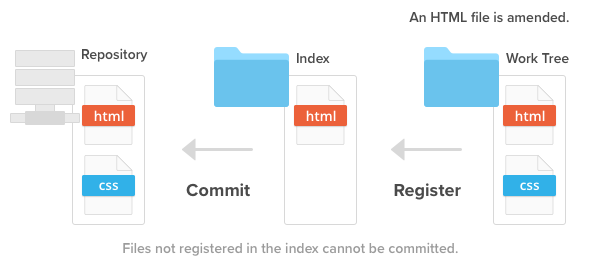
\includegraphics[scale=0.5]{images/git_workflow_001.png}
            \end{center}
            \caption{Les états des fichiers possibles}
            \label{fig:git-workflow-001}
        \end{figure}


\listoflistings
    \addcontentsline{toc}{section}{\listoflistingscaption}
\listoffigures
    \addcontentsline{toc}{section}{Table des figures}

\end{document}
